\chapter{Prototipado}
\label{prototipado}



\section{Químicos}
\paragraph{} Una vez llegados a este punto, la utilización de químicos va a comenzar. Recordar que siempre que se utilizan químicos es muy recomendado utilizar equipamiento de protección personal o EPP, guantes, gafas y bata, además de tener a mano una ducha o masa de agua para poder retirar posibles salpicaduras. Es imprescindible realizar los siguientes pasos en una habitación extremadamente ventilada, si esto no es posible, es imprescindible emplear el uso de un respirador químico de al menos \textit{A(X)BE} de clase 2 según el estándar \textit{ABEK} \cite{abek}, pues las siguientes reacciones emiten grandes cantidades de hidrógeno y otros gases aun más peligrosos, que aunque en menor cantidad, son tóxicos.

\paragraph{} A continuación se listan los químicos con los que se trabaja:

\subsection{Químicos empleados}
\paragraph{Ácido Clorhídrico al $$30\%$$} \textit{HCl} \cite{hcl}
\begin{itemize}
    \item NFPA 704: 3-0-1 \cite{nfpa704}
    \item Peligros
    \begin{itemize}
        \item Puede ser corrosivo para los metales
        \item Provoca quemaduras graves en la piel y lesiones oculares graves
        \item Puede irritar las vías respiratorias
    \end{itemize}
    \item Equipo de protección: 
    \begin{itemize}
        \item Protección ocular
        \item Protección de la piel (Goma de nitrilo > 0,3 mm)
        \item Protección respiratoria (Tipo: E \cite{abek} (Amarillo))
    \end{itemize}
\end{itemize}

\paragraph{Peróxido de Hidrógeno al $$33\%$$ (110 vol)} \textit{$$H_2O_2$$} \cite{h2o2}
\begin{itemize}
    \item NFPA 704: 3-0-3 (OX) \cite{nfpa704}
    \item Peligros
    \begin{itemize}
        \item Nocivo en caso de ingestión
        \item Provoca irritación cutánea
        \item Provoca lesiones oculares graves
        \item Nocivo en caso de inhalación
        \item Puede irritar las vías respiratorias
        \item Puede provocar perdida de consciencia
    \end{itemize}
    \item Equipo de protección: 
    \begin{itemize}
        \item Protección ocular
        \item Protección de la piel (Caucho de butilo > 0,3 mm)
        \item Protección respiratoria (Tipo: B-P2 \cite{abek} (Gris/Blanco))
    \end{itemize}
\end{itemize}

\paragraph{Hidróxido de Sodio} \textit{NaOH} \cite{naoh}
\begin{itemize}
    \item NFPA 704: 3-0-1 \cite{nfpa704}
    \item Peligros
    \begin{itemize}
        \item Puede ser corrosivo para los metales
        \item Provoca quemaduras graves en la piel y lesiones oculares graves
        \item Suspensión en el aire en forma de polvo
    \end{itemize}
    \item Equipo de protección: 
    \begin{itemize}
        \item Protección ocular
        \item Protección de la piel (Goma de nitrilo > 0,11 mm)
        \item Protección respiratoria (Tipo: P2 \cite{abek} (Blanco))
    \end{itemize}
\end{itemize}

\paragraph{Carbonato de sodio monohidrato} \textit{$$Na_2CO_3 H_2O$$} \cite{na2co3h2o}
\begin{itemize}
    \item NFPA 704: 2-0-0 \cite{nfpa704}
    \item Peligros
    \begin{itemize}
        \item Provoca irritación ocular grave
    \end{itemize}
    \item Equipo de protección: 
    \begin{itemize}
        \item Protección ocular
        \item Protección de la piel
    \end{itemize}
\end{itemize}

\paragraph{Carbonato de potasio} \textit{$$K_2CO_3$$} \cite{k2co3}
\begin{itemize}
    \item NFPA 704: 2-0-0 \cite{nfpa704}
    \item Peligros
    \begin{itemize}
        \item Provoca irritación cutánea
        \item Provoca irritación ocular grave
        \item Puede irritar las vías respiratorias
    \end{itemize}
    \item Equipo de protección: 
    \begin{itemize}
        \item Protección ocular
        \item Protección de la piel (Goma de nitrilo > 0,11 mm)
        \item Protección respiratoria (Tipo: P2 \cite{abek} (Blanco))
    \end{itemize}
\end{itemize}

\paragraph{Acetona} \textit{$$CH_3(CO)CH_3$$} \cite{acetona}
\begin{itemize}
    \item NFPA 704: 1-3-0 \cite{nfpa704}
    \item Peligros
    \begin{itemize}
        \item Provoca irritación ocular grave
        \item Líquido y vapores muy inflamables
        \item Puede provocar somnolencia o vértigo
    \end{itemize}
    \item Equipo de protección: 
    \begin{itemize}
        \item Protección ocular
        \item Protección de la piel (Caucho de butilo > 0,7 mm)
        \item Protección respiratoria (Tipo: AX \cite{abek} (Marrón))
        \item Protección antiestática
    \end{itemize}
\end{itemize}

\paragraph{alcohol isopropilico (2-propanol)} \textit{$$CH_3CH(OH)CH_3$$} \cite{isopropilico}
\begin{itemize}
    \item NFPA 704: 2-3-0 \cite{nfpa704}
    \item Peligros
    \begin{itemize}
        \item Provoca irritación ocular grave
        \item Líquido y vapores muy inflamables
        \item Puede provocar somnolencia o vértigo
    \end{itemize}
    \item Equipo de protección: 
    \begin{itemize}
        \item Protección ocular
        \item Protección de la piel (Goma de nitrilo > 0,4 mm)
        \item Protección respiratoria (Tipo: A \cite{abek} (Marrón))
        \item Protección antiestática
    \end{itemize}
\end{itemize}

\paragraph{Agua destilada} \textit{$$H_2O$$} \cite{h2o}
\begin{itemize}
    \item NFPA 704: 0-0-0 \cite{nfpa704}
    \item Peligros
    \begin{itemize}
        \item Sustancia no peligrosa
        \item Por ingestión de grandes cantidades: En caso de malestar, pedir 
atención médica
    \end{itemize}
    \item Equipo de protección: 
    \begin{itemize}
        \item Ninguno
    \end{itemize}
\end{itemize}


\subsection{Químicos producto}
\paragraph{Cloruro de cobre (I)} \textit{CuCl} \cite{cucl}
\begin{itemize}
    \item NFPA 704: 3-0-0 \cite{nfpa704}
    \item Peligros
    \begin{itemize}
        \item Nocivo en caso de ingestión o en contacto con la piel
        \item Provoca irritación cutánea
        \item Provoca lesiones oculares graves
        \item Muy tóxico para los organismos acuáticos, con efectos nocivos duraderos
    \end{itemize}
    \item Equipo de protección: 
    \begin{itemize}
        \item Protección ocular
        \item Protección de la piel (Goma de nitrilo > 0,11 mm)
        \item Protección respiratoria (Tipo: P2 \cite{abek} (Blanco))
    \end{itemize}
    \item Información adicional
    \begin{itemize}
        \item Evitar la producción de polvo
        \item Evitar su liberación al medio ambiente
        \item Mantener el producto alejado de los desagües y de las aguas superficiales y subterráneas
    \end{itemize}
\end{itemize}

\paragraph{Cloruro de cobre (II)} \textit{$$CuCl_2$$} \cite{cucl2}
\begin{itemize}
    \item NFPA 704: 2-0-1 \cite{nfpa704}
    \item Peligros
    \begin{itemize}
        \item Puede ser corrosivo para los metales
        \item Nocivo en caso de ingestión o en contacto con la piel
        \item Provoca irritación cutánea
        \item Provoca lesiones oculares graves
        \item Muy tóxico para los organismos acuáticos, con efectos nocivos duraderos
    \end{itemize}
    \item Equipo de protección: 
    \begin{itemize}
        \item Protección ocular
        \item Protección de la piel (Goma de nitrilo > 0,3 mm)
        \item Protección respiratoria (Tipo: P2 \cite{abek} (Blanco))
    \end{itemize}
\end{itemize}

\section{Herramientas de manufacturación}
\paragraph{} De forma adicional, para realizar el proceso de prototipado se han de emplear ciertas herramientas de manufacturación, estas herramientas son las siguientes:

\paragraph{Insoladora UV} una insoladora se emplea para grabar mediante luz, en este caso Ultra Violeta una imagen en un fotolito, creando un negativo de la imagen situada en la máscara utilizada para la impresión. En el caso de este proyecto, se emplea una insoladora hecha a mano que emplea cuatro tubos fluorescentes T5 en configuración 2s2p (dos sistemas en paralelo de dos tubos en serie) montados unos 70mm bajo una lamina de cristal de 4mm de grosor, espaciados uniformemente en un espacio de 220mm de anchura por el largo de tubo consumiendo en su totalidad 24W.

\paragraph{Pistola de aire caliente regulable} En el proceso de fabricación de la PCB es necesario calentar una lamina fotosensible para su correcta adhesión al cobre.

\paragraph{Rodillo de gran diámetro} para la eliminación de aire y agua en el proceso de adhesión de la anteriormente nombrada película, es necesario un rodillo de un diámetro considerable para no distorsionar el grosor de la misma.

\paragraph{Granete} Para marcar los taladros necesarios en la placa, ya sean para vías o componentes tht.

\paragraph{Taladro o micro-taladro} Para realizar los taladros en la placa.

\section{Herramientas de ensamblado}
\paragraph{}


\paragraph{} Es imprescindible también realizar un desecho responsable de los materiales tóxicos generados, en nuestro caso cloruro de cobre (I y II), los cuales son altamente contaminantes a la fauna marina.

\paragraph{}
La etapa de prototipado es esencial

\paragraph{}
Para el proceso de prototipado se realizará uso del programa de diseño asistido por ordenador \textit{kicad} \cite{kicad} para generar tanto el esquema electrónico como el diseño de la placa para finalmente manufacturar y grabar mediante ácido la placa PCB donde se soldarán todos los componentes

\paragraph{} En este capitulo se mostrará dicho proceso de inicio a fin, desde las pruebas de insolación, revelado y grabado, hasta el diseño y realización de la placa final operativa.

\section{Objetivo}

\section{Proceso fotolítico}
\subsection{Introducción}
\paragraph{} Para la realización de circuitos impresos, un proceso químico que ataca el cobre es usado, pero este proceso aplicado a una placa de cobre convencional resulta en el ataque de todo el cobre, obteniendo una placa totalmente limpia del metal en cuestión. Sin embargo, si empleamos alguna máscara resistente al agente atacante, podemos diferenciar distintas zonas en las que el cobre no será atacado. Combinando esta técnica con las extremadamente buenas características conductoras del cobre, podemos impresionar pistas conductoras de cobre para el conexionado de nuestra implementación del circuito anteriormente diseñado en el capítulo \ref{diseño_hardware}.

\paragraph{} Para la obtención de dicha mascara, podemos realizar uso de nuevo de \textit{KiCad} \cite{kicad}.

\paragraph{} La mascara en cuestión es una película fotosensible a base de resina \cite{douglas} la cual se compone de una resina azulada protegida en ambas caras por protectores plásticos tal y como se observa en la figura \ref{fig:tfg:06:capas_pelicula}.

\paragraph{} Este compuesto cambia de composición una vez expuesto a luz ultravioleta también llamada luz UV, el cambio es visible también, oscureciéndose en el cambio, véanse figuras \ref{fig:tfg:06:pelicula_sin_insolar} y \ref{fig:tfg:06:pelicula_insolada}.

\paragraph{} Si exponemos la película utilizando una mascara impresa en papel de cebolla o acetato, podemos exponer selectivamente zonas de esta, creando zonas expuestas y zonas sin exponer, estas zonas expuestas son resistentes al químico revelador, mientras que las zonas no expuestas son fácilmente atacadas por el revelador.

\begin{figure}[!htb]
    \centering
    \begin{subfigure}[b]{.475\textwidth}
        \centering
        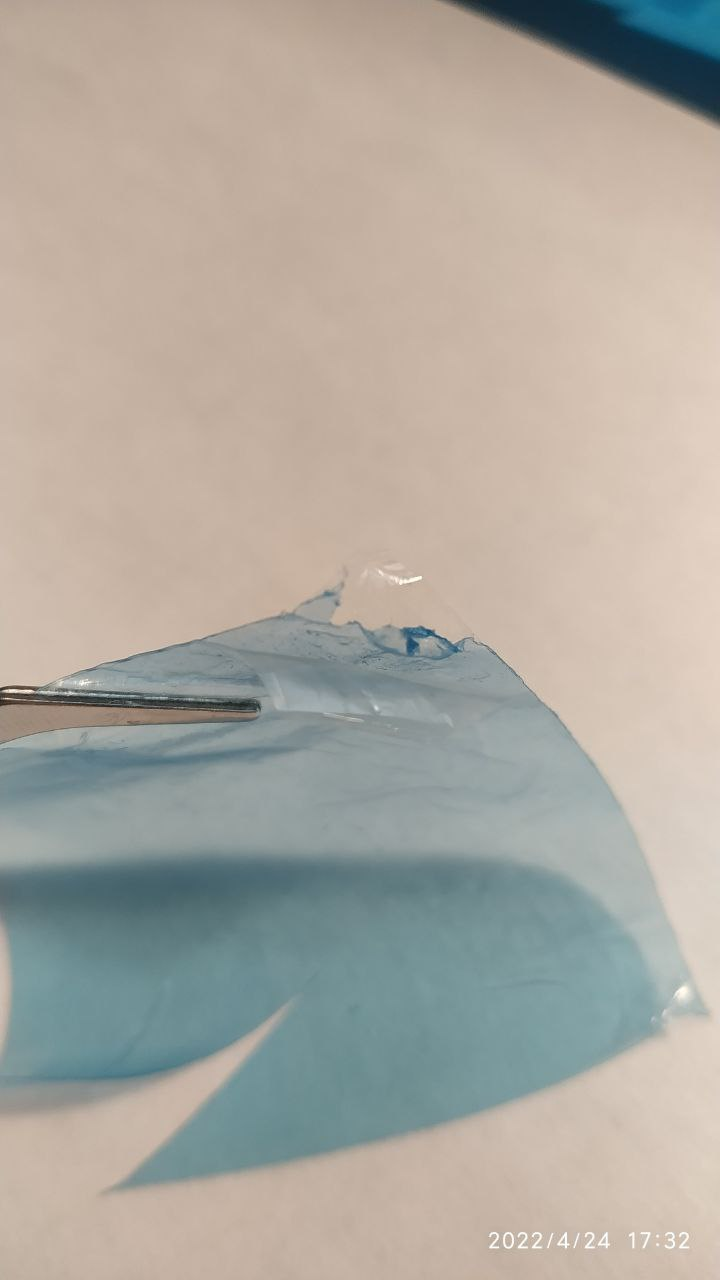
\includegraphics[width=1\textwidth, trim={0 400 0 400}, clip]{tfg/figuras/06_prototipado/explicacion/pelicula_seca_capas.png}
        \caption{película fotosensible en azul y sus dos capas protectoras}
        \label{fig:tfg:06:capas_pelicula}
    \end{subfigure}%
    \hfill
    \begin{subfigure}[b]{.475\textwidth}
    \centering
        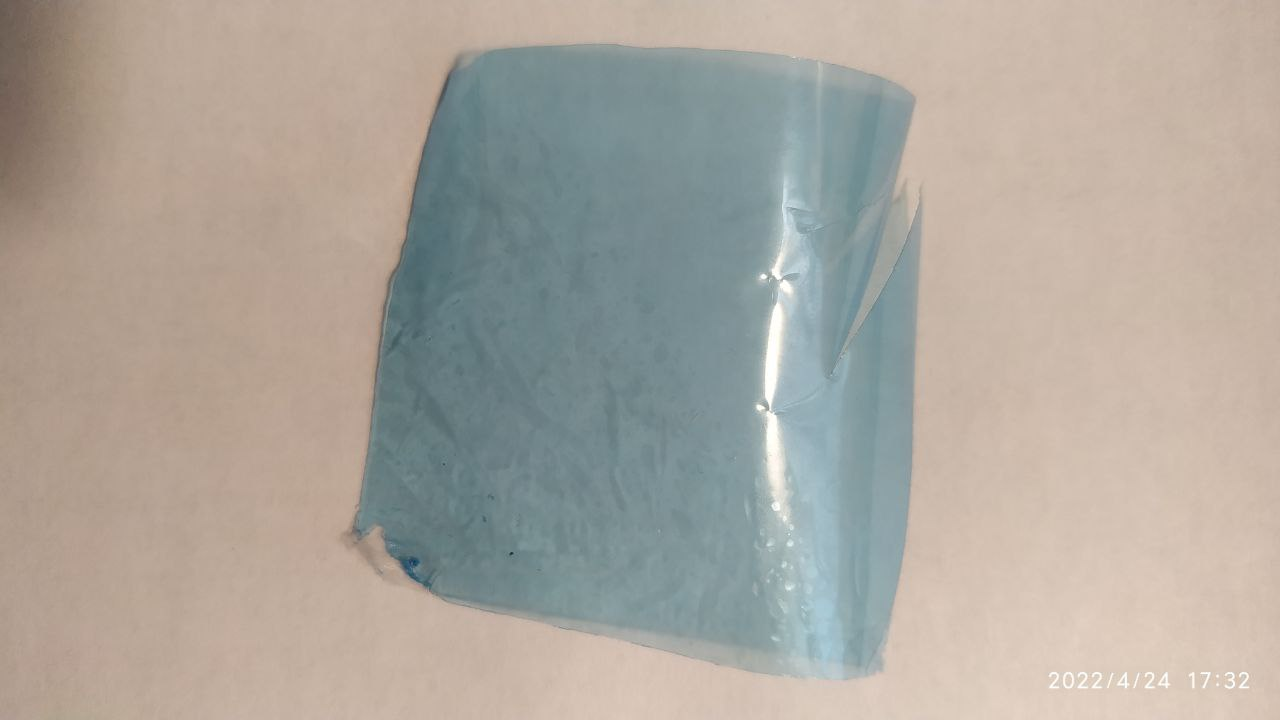
\includegraphics[width=1\textwidth, trim={150 65 150 0}, clip]{tfg/figuras/06_prototipado/explicacion/pelicula_seca_sin_insolar.png}
        \caption{Película sin insolar}
        \label{fig:tfg:06:pelicula_sin_insolar}
    \end{subfigure}
    \vskip\baselineskip
    \begin{subfigure}[b]{.475\textwidth}
        \centering
        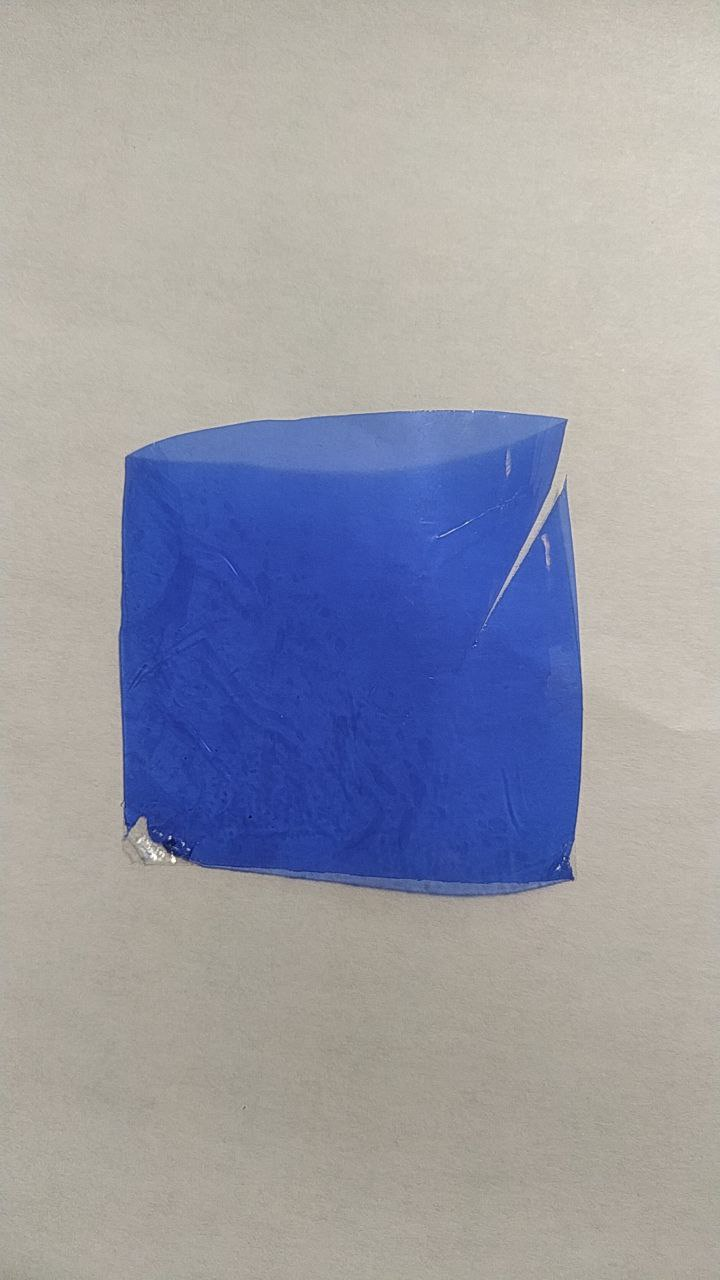
\includegraphics[width=1\textwidth, trim={0 400 0 400}, clip]{tfg/figuras/06_prototipado/explicacion/pelucula_seca_expuesta.png}
        \caption{Película tras exposición a luz ultravioleta}
        \label{fig:tfg:06:pelicula_insolada}
    \end{subfigure}%
    \caption{Película fotosensible}
    \label{fig:tfg:06:pelucila_fotosensible}
\end{figure}

\pagebreak

\subsection{Preparación de placa}

\paragraph{} Antes de realizar cualquier acción a la placa de cobre, es necesario remover tanto oxido como sea posible para la correcta aplicación de la película fotosensible. Unos de los métodos más populares es la abrasión mediante lana de acero, sin embargo, en mi opinión, es demasiada abrasión dejando depresiones de gran profundidad en el cobre, dificultando la correcta adhesión de la película. Si un simple estropajo de cocina abrasivo (normalmente color verde) es usado, la superficie del cobre queda suficientemente limpia y con imperfecciones no demasiado profundas que contribuyen a la correcta aplicación de la película.

\paragraph{} Movimientos circulares y algo erráticos del estropajo durante la limpieza crean un entramado de imperfecciones, que según la experimentación dan los mejores resultados.

\paragraph{} Es necesario erosionar la superficie hasta obtener resultados similares a la figura \ref{fig:tfg:06:placa_de_cobre_tratada} y limpiarla con algún disolvente como acetona para eliminar cualquier grasa o partículas.

\paragraph{} Una seria de baños de limpieza han de ser realizados, primero, un baño de hidróxido de sodio será empleado para eliminar cualquier material orgánico, normalmente residuos grasos. Posteriormente, un baño de ácido clorhídrico el cual tiene el objetivo de eliminar la capa de oxido del cobre. 

\begin{figure}[!htb]
    \centering
    \begin{subfigure}[b]{.475\textwidth}
        \centering
        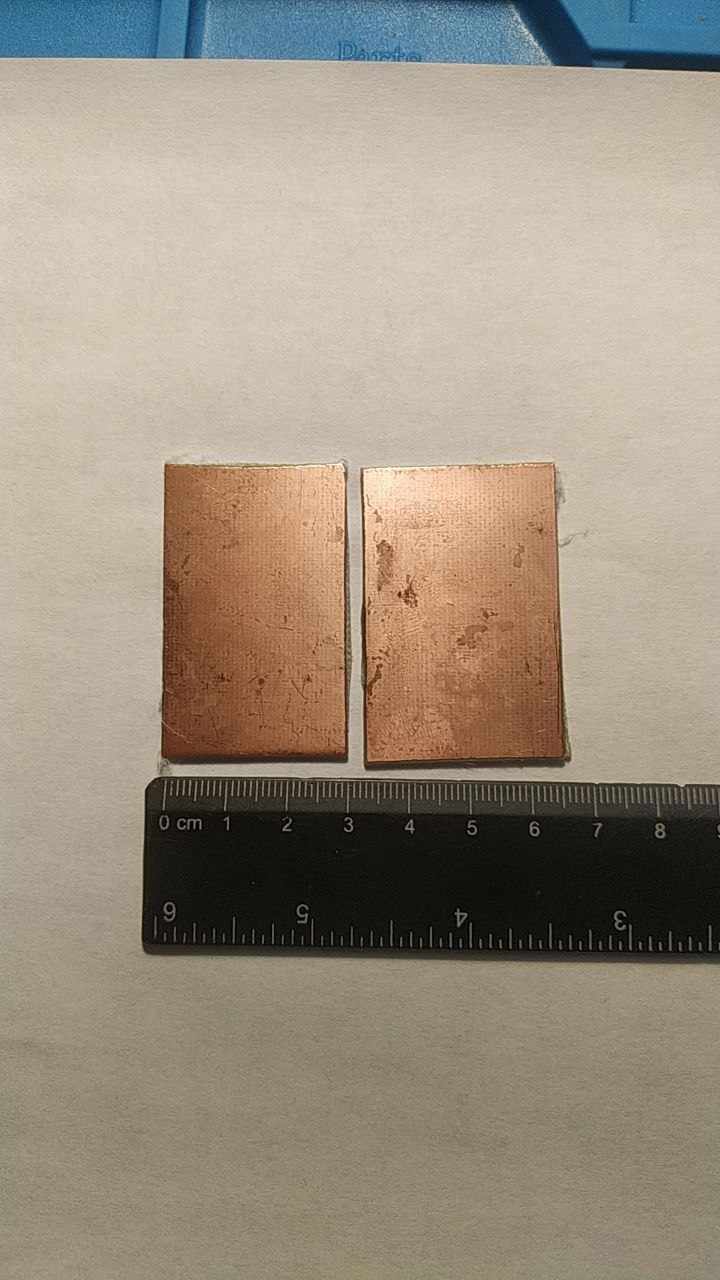
\includegraphics[width=1\textwidth, trim={0 400 0 400}, clip]{tfg/figuras/06_prototipado/limpiado/cobre_sin_tratar.png}
        \caption{Placas de cobre sin tratar}
        \label{fig:tfg:06:placa_de_cobre_sin_tratar}
    \end{subfigure}
    \hfill
    \begin{subfigure}[b]{.475\textwidth}
        \centering
        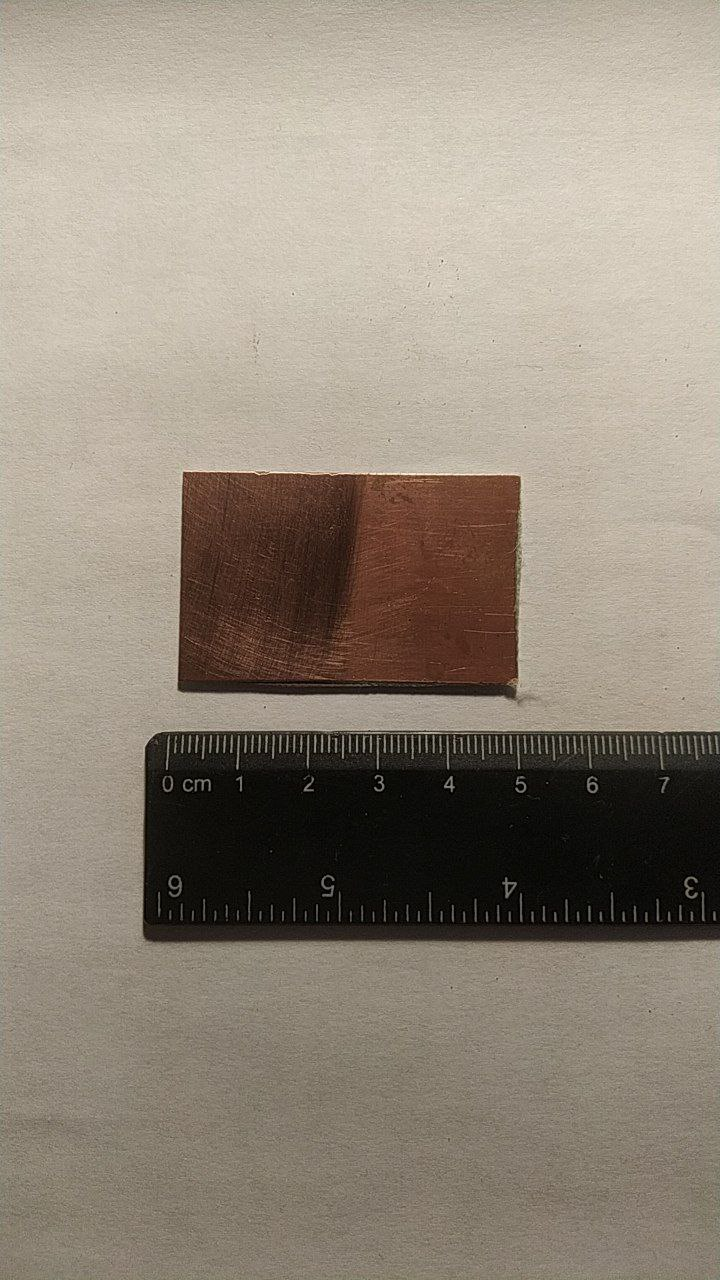
\includegraphics[width=1\textwidth, trim={0 400 0 400}, clip]{tfg/figuras/06_prototipado/limpiado/cobre_medio_tratar.png}
        \caption{Placa de cobre a medio limpiar}
        \label{fig:tfg:06:placa_de_cobre_medio_tratar}
    \end{subfigure}
    \vskip\baselineskip
    \begin{subfigure}[b]{.475\textwidth}
        \centering
        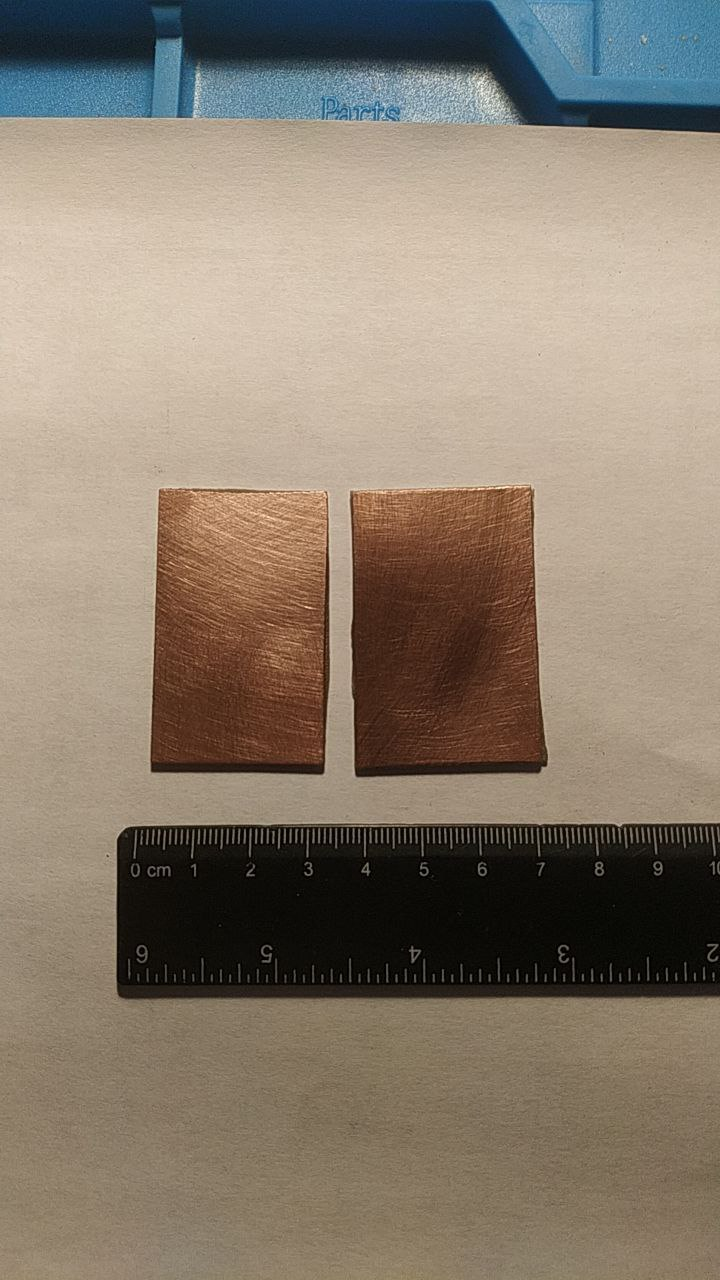
\includegraphics[width=1\textwidth, trim={0 350 0 450}, clip]{tfg/figuras/06_prototipado/limpiado/cobre_tratado.png}
        \caption{Placas de cobre tras el limpiado}
        \label{fig:tfg:06:placa_de_cobre_tratada}
    \end{subfigure}%
    \hfill
    \begin{subfigure}[b]{.475\textwidth}
        \centering
        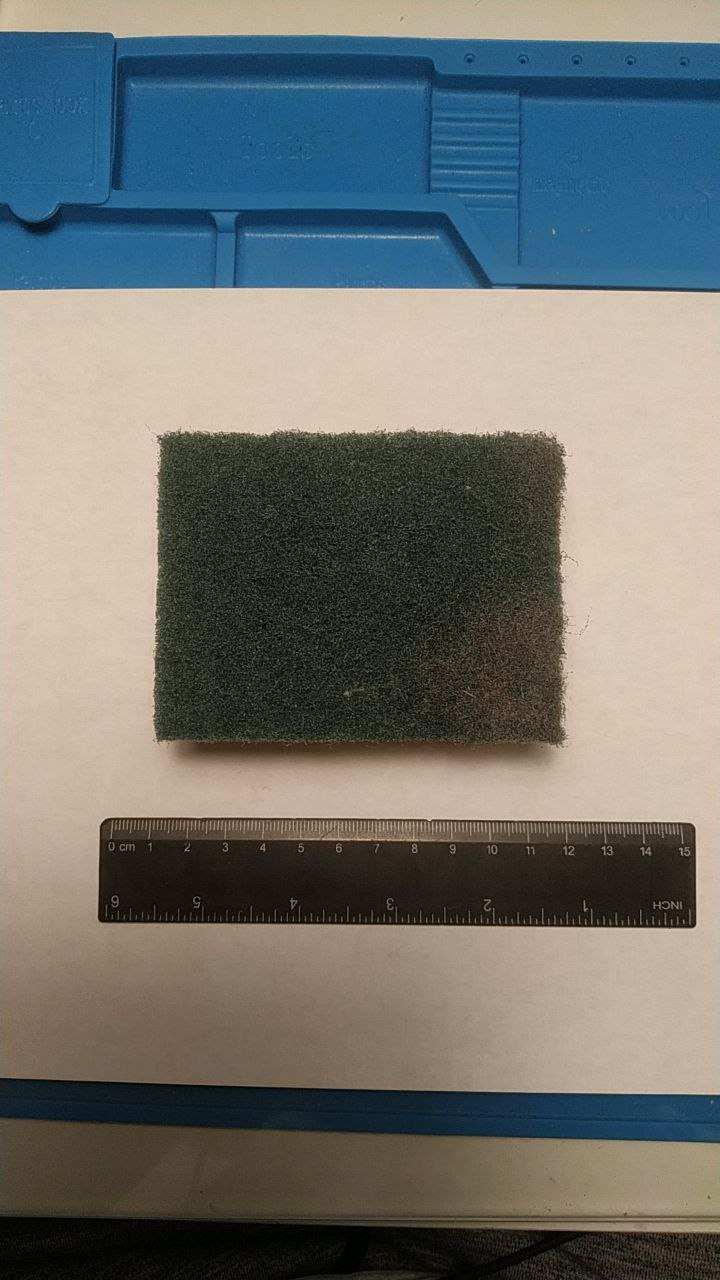
\includegraphics[width=1\textwidth, trim={0 400 0 400}, clip]{tfg/figuras/06_prototipado/limpiado/estropajo.png}
        \caption{Estropajo abrasivo usado para la limpieza}
        \label{fig:tfg:06:estropajo}
    \end{subfigure}%
    \caption{Proceso de limpieza de placa de cobre}
    \label{fig:tfg:06:tratamiento_cobre}
\end{figure}

\pagebreak

\paragraph{} Una vez tenemos el cobre limpio, podemos proceder a la aplicación de la película fotosensible. Esto es realizado retirando una de las dos capas protectoras y aplicándola sobre la placa de cobre limpio y con la ayuda de agua, preferiblemente destilada. La aplicación debe de ser similar al proceso de instalación de un protector de pantalla de teléfono móvil, sin dejar ninguna burbuja de aire.

\paragraph{} Tras la aplicación, se ha de extraer todo el agua posible y aplicar calor, seguido de presión lo mas uniforme posible para no dañar la película y crear imperfecciones. Esto es realizado mediante el aire caliente de una estación de soldadura a 115Cº y moviendo el foco de calor por toda la placa de la forma uniforme. 

\paragraph{} Otras opciones populares son una laminadora de papel, o una simple plancha al mínimo de temperatura. Ambas de estas opciones aplican ya presión, cosa que el aire caliente no, por esto es necesario presionar la película con un objeto plano o un rodillo. Este proceso esta ilustrado en la figura \ref{fig:tfg:06:aplicacion_pelicula}.

\paragraph{} Para retirar las capas protectoras es útil utilizar un par de cortes de cinta adhesiva, retirándolas realizando la fuerza en la misma dirección y sentido opuesto, posicionando la película en la misma dirección, esto facilitará la retirada de la capa protectora a la que la cinta adhesiva con el mismo sentido que la película esta adherida.

\paragraph{} Es importante minimizar la película a luces intensas, de esta manera, el revelador será más efectivo.

\paragraph{} Una vez retirada una de las capas protectoras la aplicaremos sobre la placa de cobre tal y como se menciona en los párrafos anteriores.

\pagebreak

\begin{figure}[!htb]
    \centering
    \begin{subfigure}[b]{.475\textwidth}
        \centering
        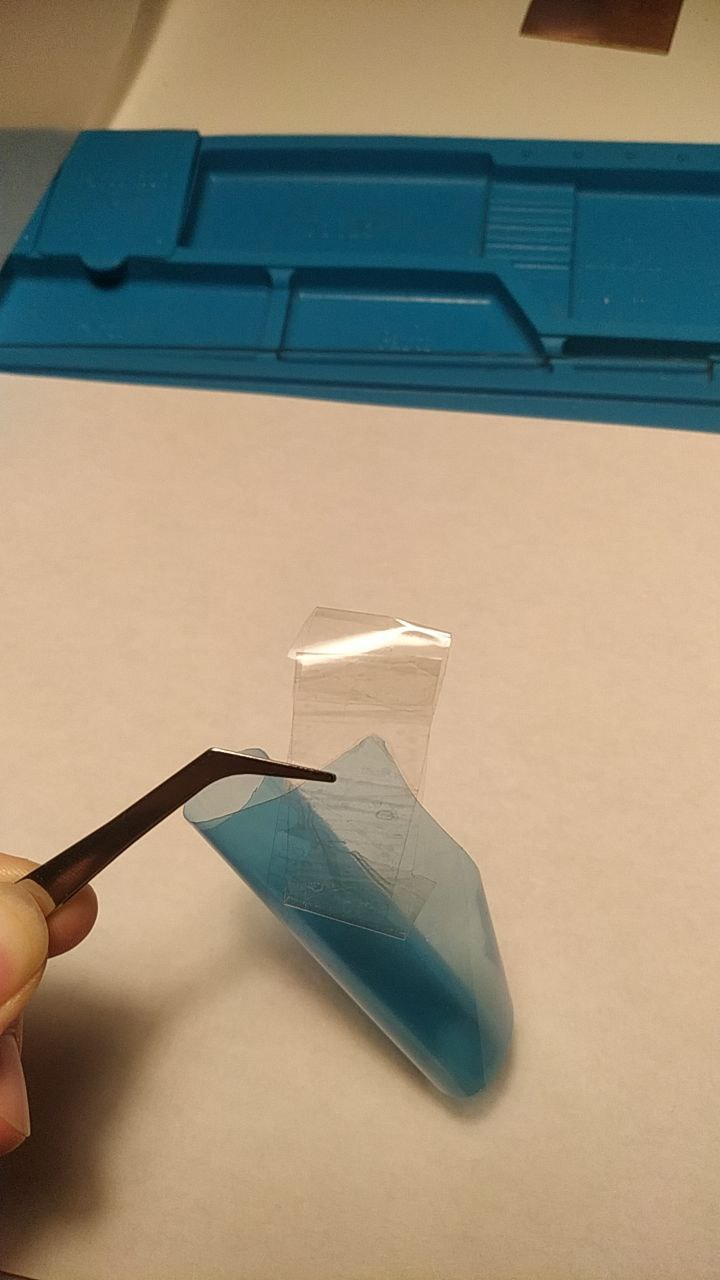
\includegraphics[width=1\textwidth, trim={0 400 0 500}, clip]{tfg/figuras/06_prototipado/pelicula/separacion_protector_1.png}
        \caption{La cinta adhesiva facilita la separación del protector}
        \label{fig:tfg:06:separacion_1}
    \end{subfigure}
    \hfill
    \begin{subfigure}[b]{.475\textwidth}
        \centering
        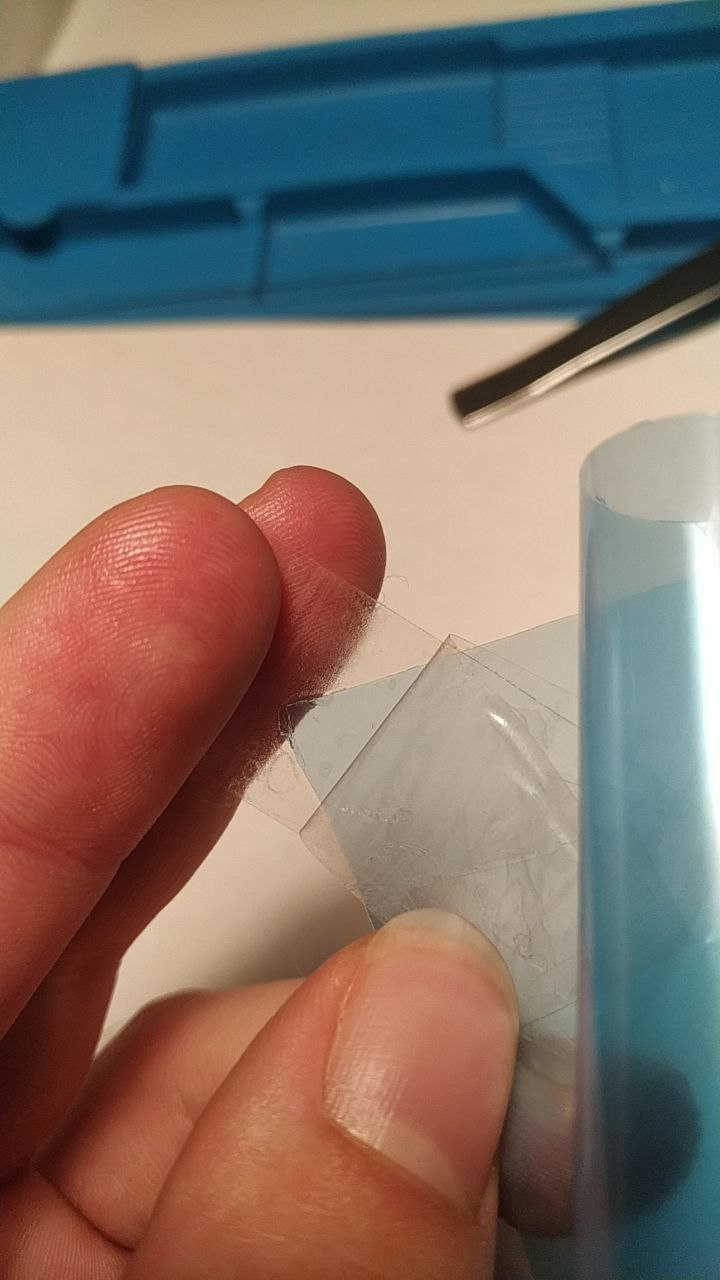
\includegraphics[width=1\textwidth, trim={0 400 0 500}, clip]{tfg/figuras/06_prototipado/pelicula/separacion_protector_2.png}
        \caption{Separación de protector interno}
        \label{fig:tfg:06:separacion_2}
    \end{subfigure}
    \vskip\baselineskip
    \begin{subfigure}[b]{.475\textwidth}
        \centering
        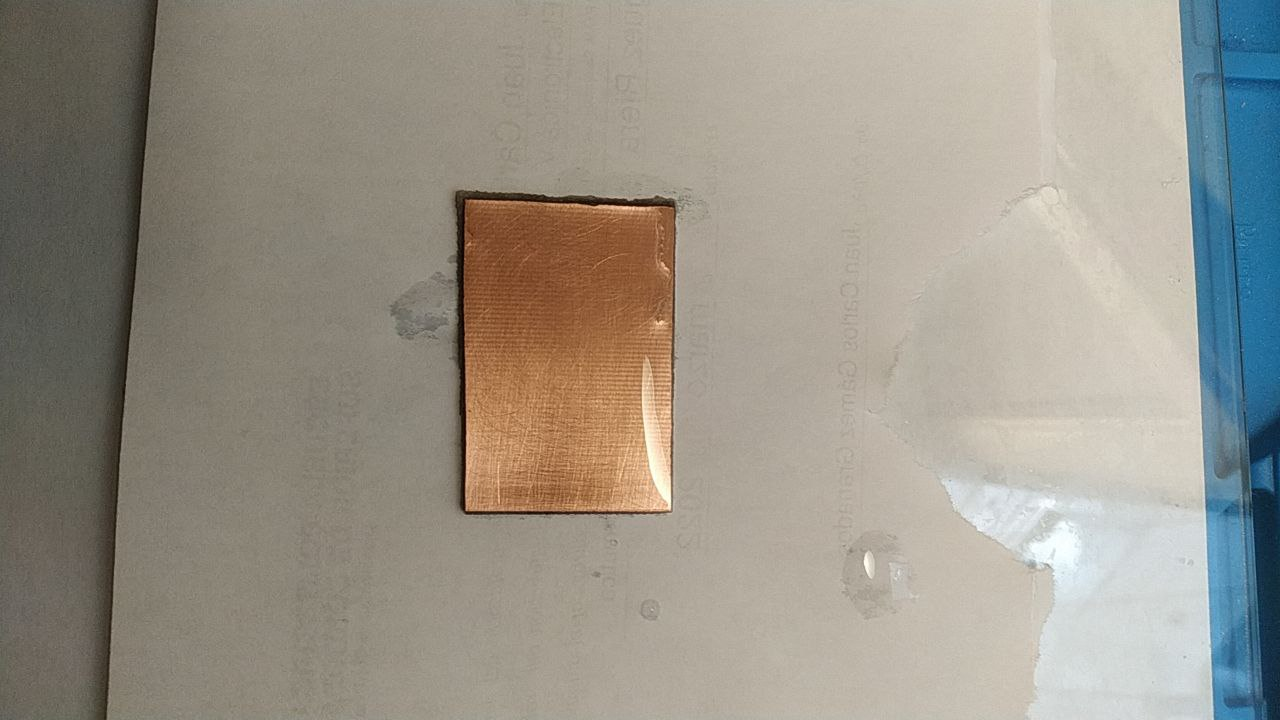
\includegraphics[width=1\textwidth, trim={100 100 200 100}, clip]{tfg/figuras/06_prototipado/pelicula/agua_placa.png}
        \caption{El agua facilita la aplicación de la película}
        \label{fig:tfg:06:agua}
    \end{subfigure}%
    \hfill
    \begin{subfigure}[b]{.475\textwidth}
        \centering
        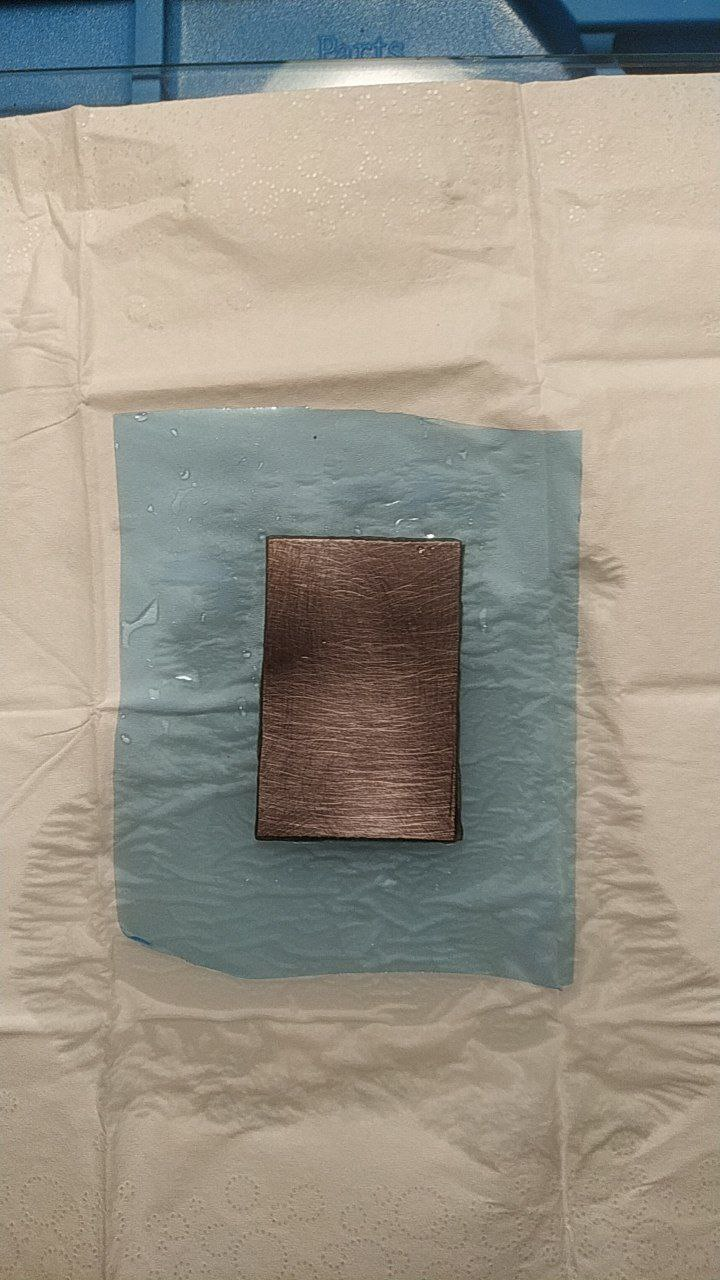
\includegraphics[width=1\textwidth, trim={0 400 0 500}, clip]{tfg/figuras/06_prototipado/pelicula/placa_y_film.png}
        \caption{Comprobación de burbujas de aire}
        \label{fig:tfg:06:film_en_placa}
    \end{subfigure}%
   \vskip\baselineskip
    \begin{subfigure}[b]{.475\textwidth}
        \centering
        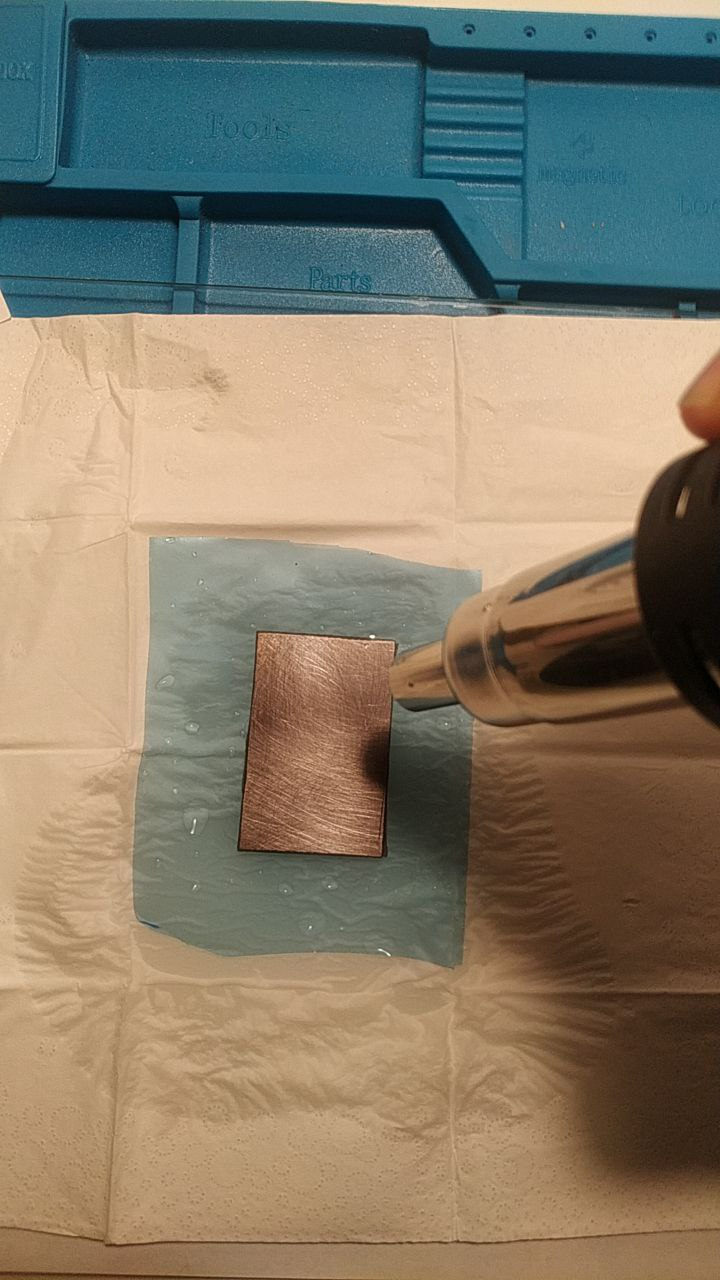
\includegraphics[width=1\textwidth, trim={0 400 0 500}, clip]{tfg/figuras/06_prototipado/pelicula/aire_caliente.png}
        \caption{Aire caliente calentando la película fotosensible}
        \label{fig:06:aire}
    \end{subfigure}%
    \hfill
    \begin{subfigure}[b]{.475\textwidth}
        \centering
        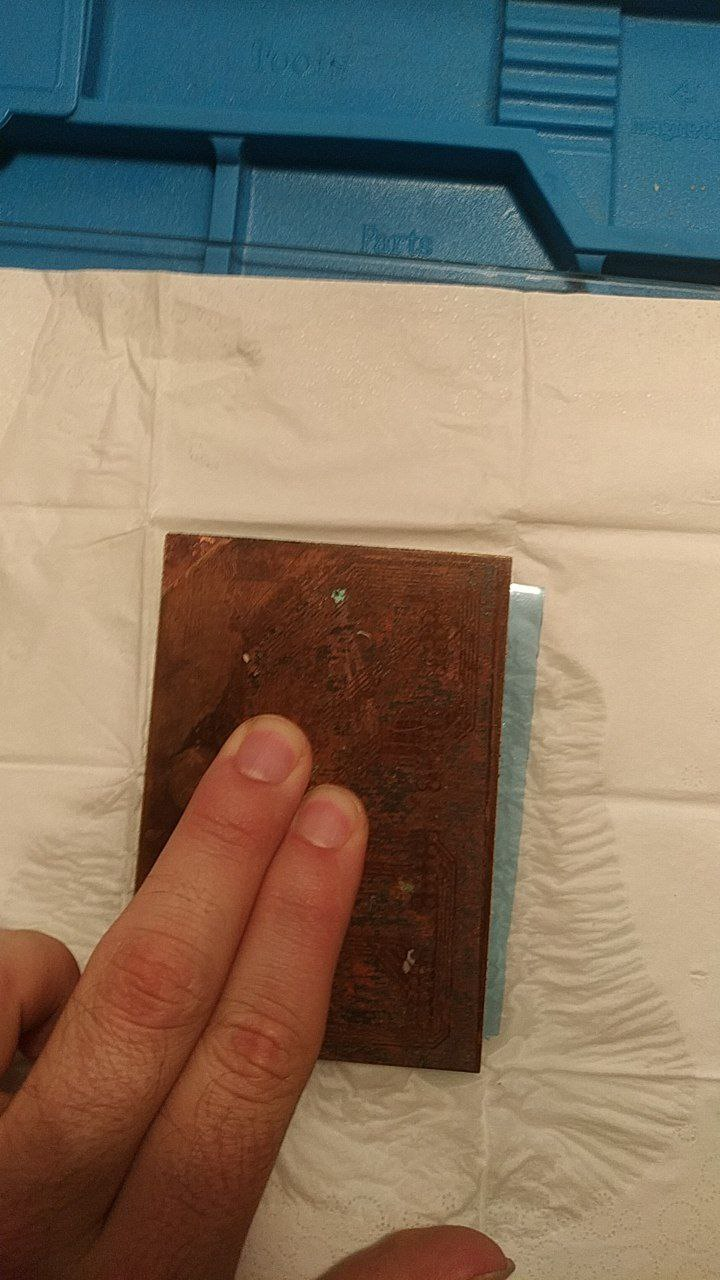
\includegraphics[width=1\textwidth, trim={0 400 0 500}, clip]{tfg/figuras/06_prototipado/pelicula/presion.png}
        \caption{Aplicación de presión}
        \label{fig:tfg:06:presion}
    \end{subfigure}%
    \vskip\baselineskip
    \begin{subfigure}[b]{.475\textwidth}
        \centering
        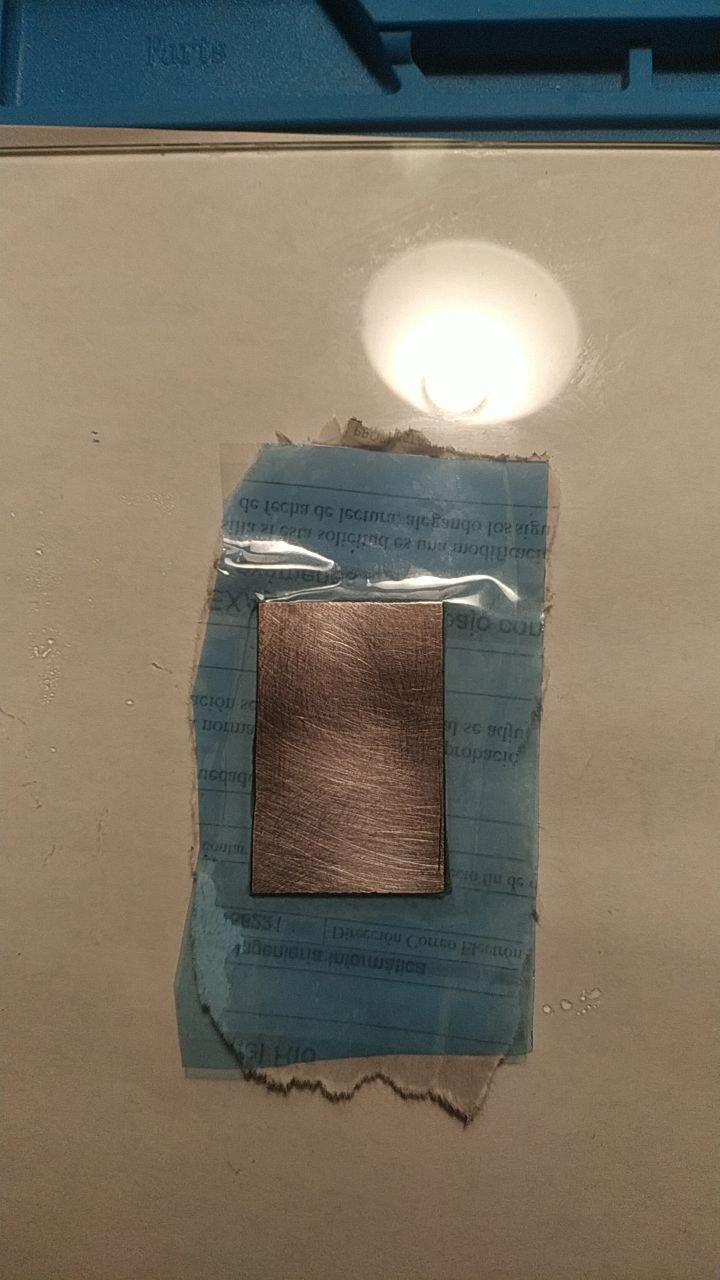
\includegraphics[width=1\textwidth, trim={0 350 0 550}, clip]{tfg/figuras/06_prototipado/pelicula/placa_con_film_pegado.png}
        \caption{Placa de cobre con película fotosensible adherida}
        \label{fig:tfg:06:placa_con_film_pegado}
    \end{subfigure}%
    \caption{Proceso de aplicación de película fotosensible}
    \label{fig:tfg:06:aplicacion_pelicula}
\end{figure}

\pagebreak
\subsection{Insolación}

\paragraph{} Antes de la insolación, la película ha de reposar durante al menos quince (15) minutos en total oscuridad para su correcta adhesión. Una vez adherida correctamente, podemos proceder a la insolación. 

\paragraph{} Para ello, utilizaremos cualquier fuente de luz ultravioleta, en nuestro caso, una insoladora de 4 Tubos fluorescentes T5 de 8W cada uno a una distancia aproximada del plano receptor de 6cm es utilizada (véase figura \ref{fig:tfg:06:insoladora})


\begin{figure}[!htb]
    \centering
    \begin{subfigure}[b]{.475\textwidth}
        \centering
        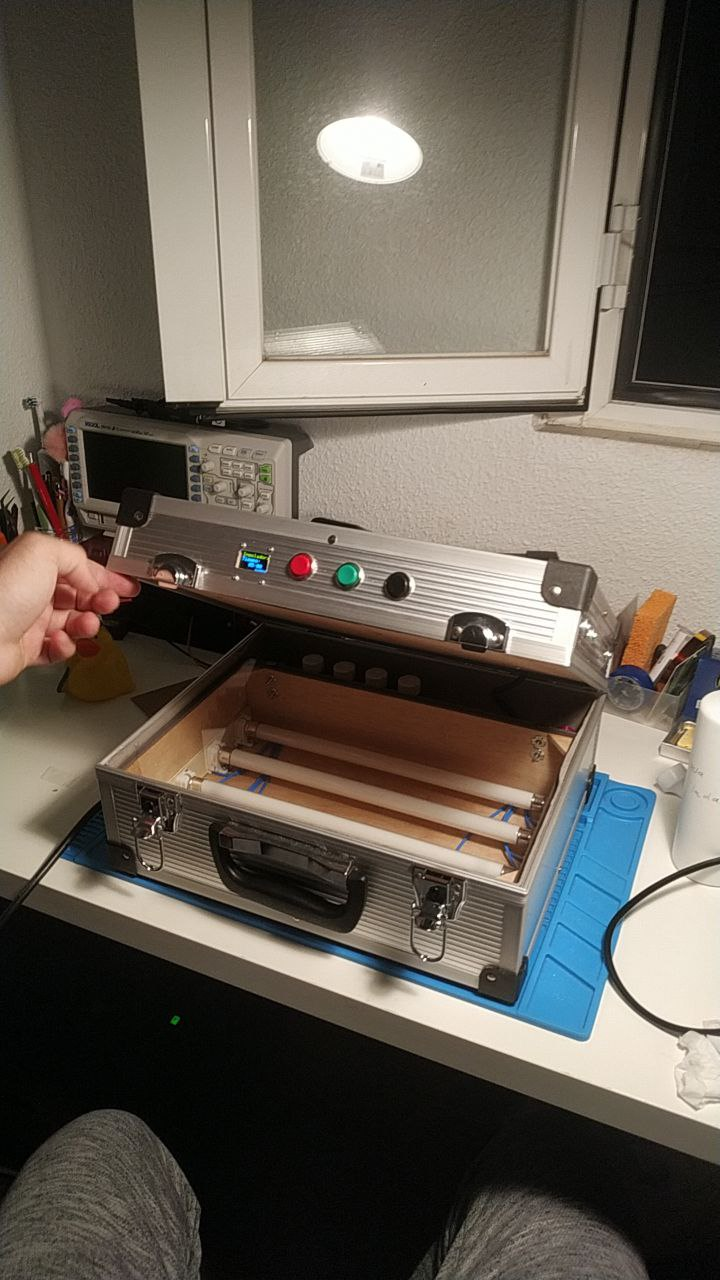
\includegraphics[width=1\textwidth, trim={0 400 0 500}, clip]{tfg/figuras/06_prototipado/insolacion/insoladora.png}
        \caption{Insoladora}
        \label{fig:tfg:06:insoladora}
    \end{subfigure}
    \hfill
    \begin{subfigure}[b]{.475\textwidth}
        \centering
        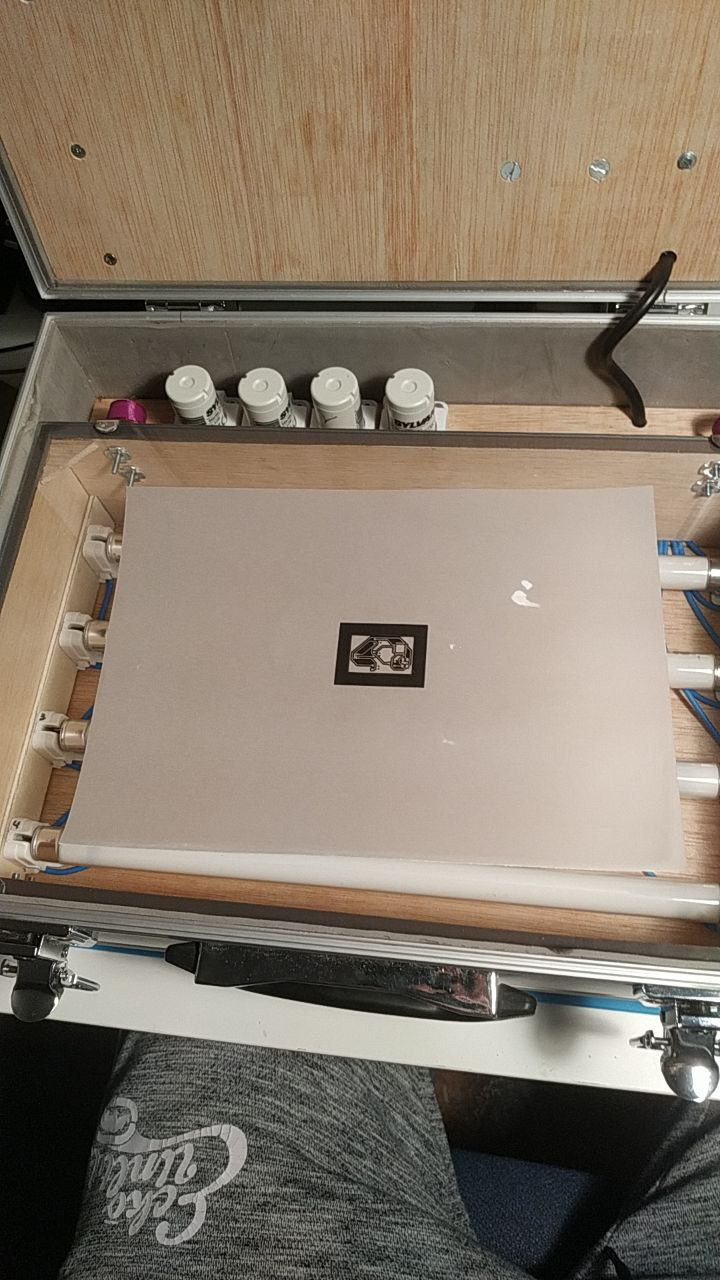
\includegraphics[width=1\textwidth, trim={0 400 0 500}, clip]{tfg/figuras/06_prototipado/insolacion/fotolito.png}
        \caption{Posicionamiento de la mascara}
        \label{fig:tfg:06:fotolito}
    \end{subfigure}
    \vskip\baselineskip
    \begin{subfigure}[b]{.475\textwidth}
        \centering
        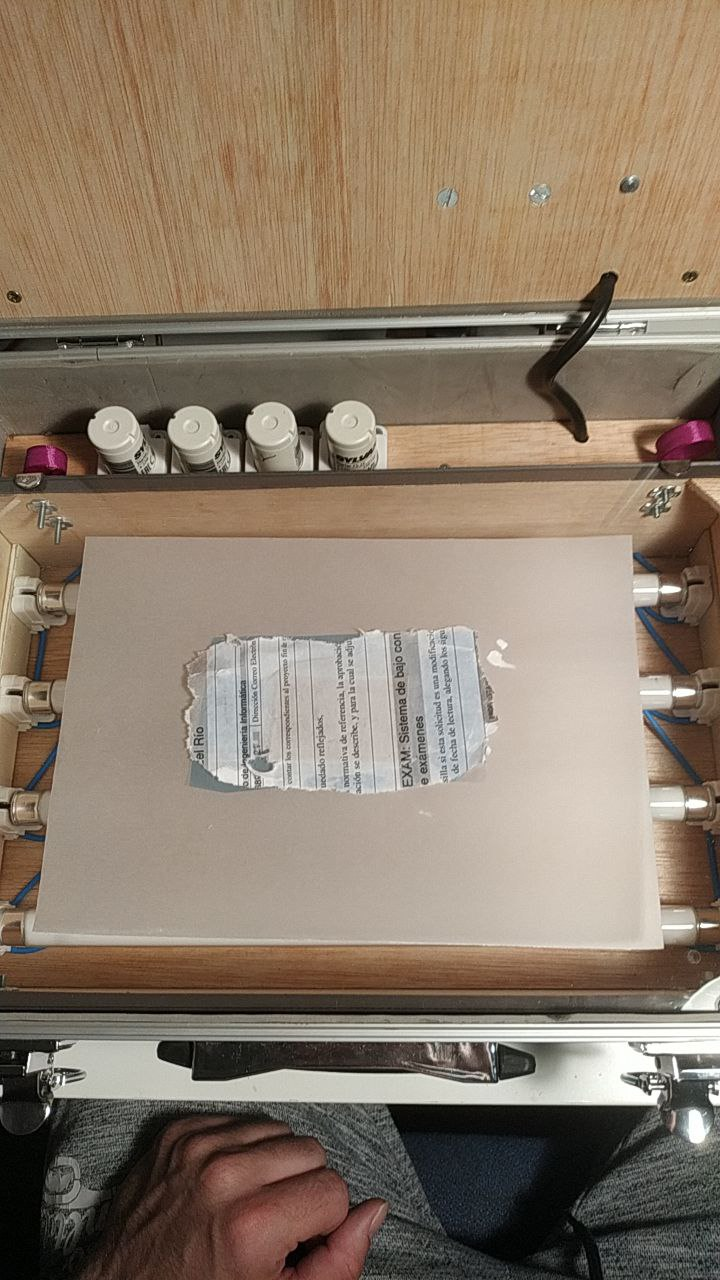
\includegraphics[width=1\textwidth, trim={0 400 0 500}, clip]{tfg/figuras/06_prototipado/insolacion/placa_sobre_fotolito.png}
        \caption{Placa con película fotosensible o fotolito sobre mascara}
        \label{fig:tfg:06:placa_en_fotolito}
    \end{subfigure}%
    \hfill
    \begin{subfigure}[b]{.475\textwidth}
        \centering
        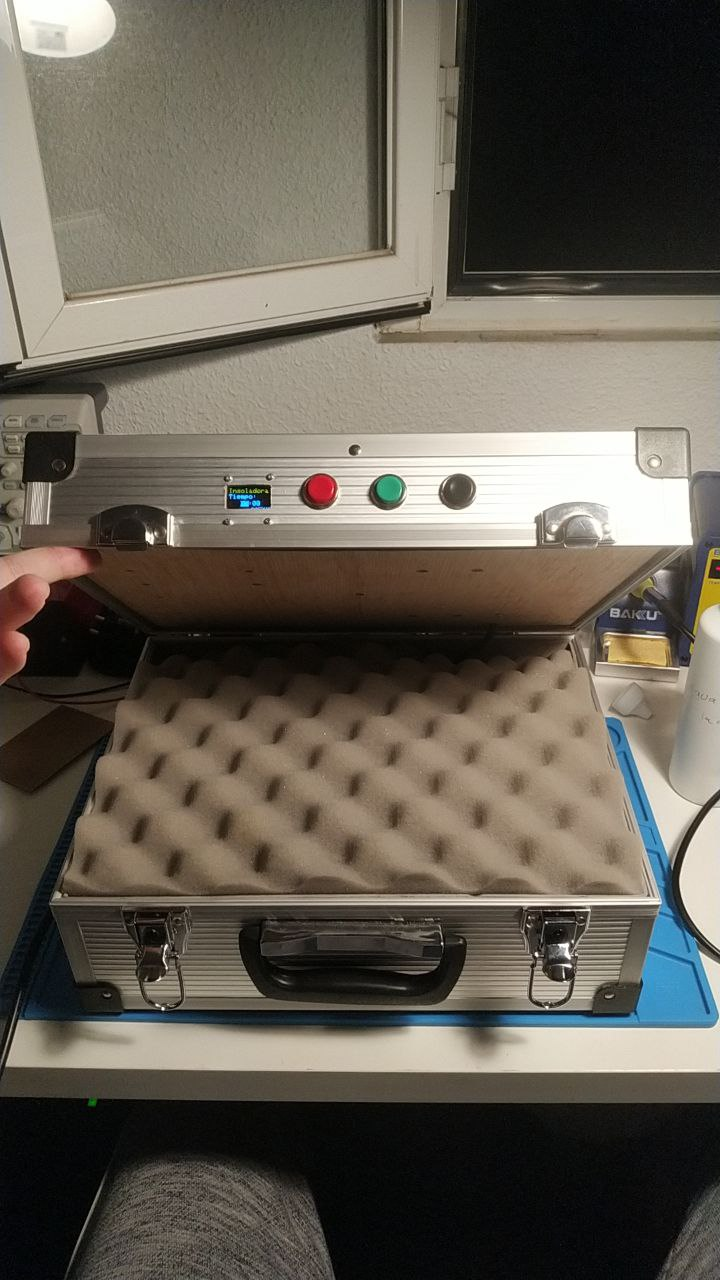
\includegraphics[width=1\textwidth, trim={0 400 0 500}, clip]{tfg/figuras/06_prototipado/insolacion/fotolito_plano.png}
        \caption{Espuma para aplanar la columna mascara/fotolito durante insolación}
        \label{fig:tfg:06:placa_en_fotolito}
    \end{subfigure}%
    \vskip\baselineskip
    \begin{subfigure}[b]{.475\textwidth}
        \centering
        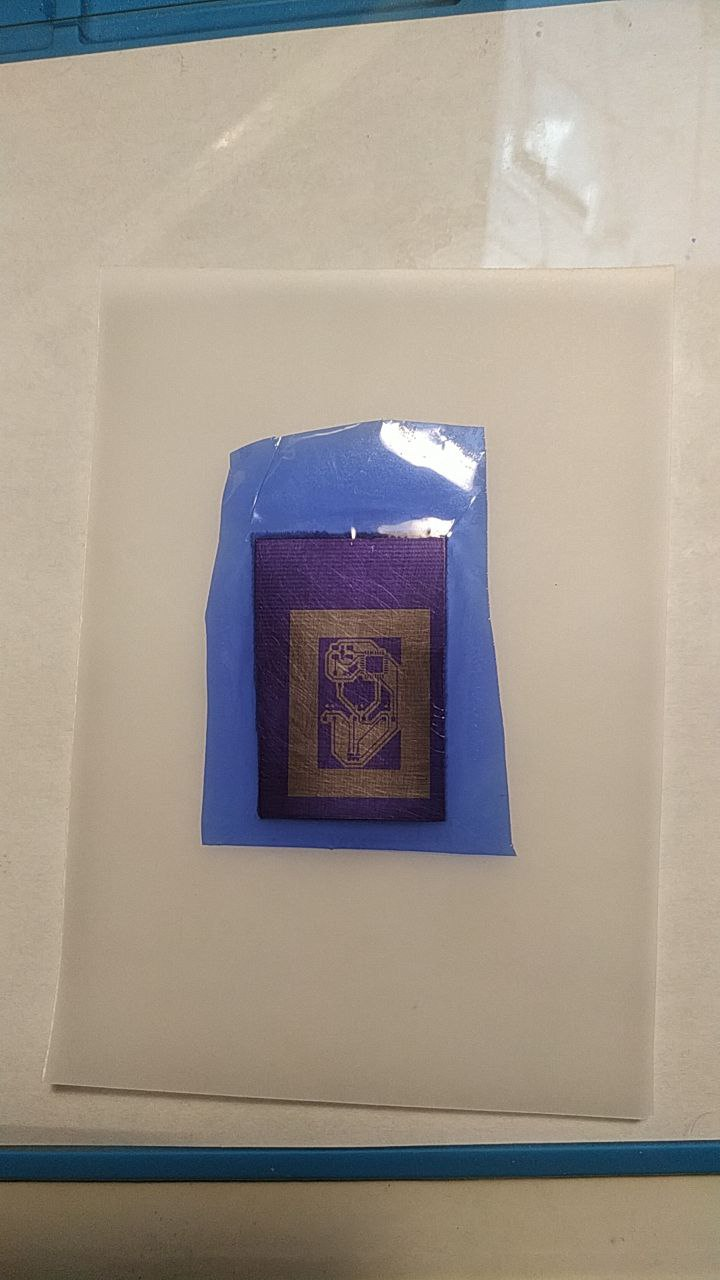
\includegraphics[width=1\textwidth, trim={0 400 0 500}, clip]{tfg/figuras/06_prototipado/insolacion/resultado_insolacion.png}
        \caption{Resultados de la insolación tras un minuto y diez segundos}
        \label{fig:tfg:06:resultado_insolacion}
    \end{subfigure}%
    \caption{Proceso de insolación}
    \label{fig:tfg:06:aplicacion_pelicula}
\end{figure}


\pagebreak


\paragraph{} El proceso de insolación se realiza durante treinta (30) segundos. Este tiempo varará dependiendo de la intensidad de la luz ultravioleta.

\paragraph{} Si alguna parte del circuito es especialmente complicada, se recomienda que se posicione directamente sobre un tubo ultravioleta, creando así pistas con mayor resolución.

\subsection{Revelado}

\paragraph{} Para disolver la película no expuesta, podemos usar una disolución de \textit{carbonato potásico} ($K_2CO_3$) al 5\% en agua por peso, esta puede ser del grifo. Este baño se realizará hasta que se retire toda la película no expuesta, los tiempos variarán mucho en función de la temperatura del baño, pero estos rondan normalmente los tres (3) minutos en una temperatura normal de interior.

\paragraph{} El retirado de la lamina superior se ha de realizar justo antes de este baño revelador para minimizar la exposición de la película al oxigeno y así evitar la oxidación.

\paragraph{} Durante el baño de bases podemos ayudarnos de un pincel o una esponja suave para retirar de película disuelta, pero esto se realiza únicamente a partir de los dos (2) minutos, esta acción se realiza para evaluar la progresión del baño.

\paragraph{} El revelado sera completado cuando una vez aclarada la placa con agua y estando completamente seca, se pueda observar que no existe película no disuelta entre las pistas o contactos ni tampoco flecos de película en los laterales de las mismas pistas que puedan interferir en el proceso de ataque ácido.

\subsection{Ataque ácido}

\paragraph{} El ataque ácido se realizará en un baño al 50\% ácido clorhídrico y 50\% peróxido de hidrógeno, es importante que ambos sean al menos de 20\% en conentración, puesto que si no la mezcla contendrá demasiado poco componente atacante y la reacción será muy lenta.

\paragraph{} Tampoco se recomienda usar nada por encima del 40\%, sobre todo de peróxido de hidrógeno, puesto que puede causar graves quemaduras químicas e incluso potenciar la combustión de materiales inflamables, creando un riesgo de explosión.

\paragraph{} Este baño no debe durar más de dos (2) minutos, puesto que las pistas sobre expuestas al baño químico se verán reducidas en su anchura, pudiendo provocar cortes en las mismas.

\subsection{Eliminación de película protectora}

\paragraph{} Una exposición de alguna base más potente como el hidróxido sódico ($NaOH$) al 1\% puede ser de ayuda para retirar la película de las pistas y contactos de la placa final.
